\documentclass[11pt]{article}
\usepackage{graphicx}
\usepackage{caption}
\usepackage{subfig}
\usepackage{geometry}
\usepackage{amsfonts}
\usepackage{amsmath}
\newcommand{\abs}[1]{\lvert #1 \rvert}
\usepackage{indentfirst}
\geometry{letterpaper, portrait, margin=1in}
\setlength{\parindent}{0cm}
\begin{document}

\setlength\parindent{24pt}

\begin{center}
Project summary

\null

Matthew LeDuc

\null

625.721 Final Project Proposal and Progress
\end{center}

\section{Proposal}
For my final project, I have decided to attempt to develop a realistic model of wind direction time series in the Atlantic Ocean. My data that I will compare to will come from the National Data Buoy Center which contains data of wind direction at buoy locations in the Atlantic and Pacific Ocean that is updated every hour. 
It also, should I decide to add on to my project, contains data for wind speed and wave height and direction. 

Directional data like what I am analyzing is not as well-behaved as more typical types of data because it does not exist on a nice set like $\mathbb{R}^n$ or $\mathbb{Z}$. This data is drawn from the interval $[0,360)$, which is complicated because $0$ degrees and $360$ degrees are the same angle, and therefore $1$ degree is as far from $0$ as $359$ is. There has been a large amount of work done on the analysis and modeling of this type of data, see for example \cite{fisher}, \cite{Craig}, and \cite{Kaito}. There are several distributions that can be used to model this data, however I have decided to use the Von Mises distribution, which is related to the normal distribution. It is given by 

\begin{equation}
f(x) = \frac{e^{\kappa \cos{(x-\mu)}}}{2\pi I_0(\kappa)}
\end{equation}

where $I_0(x)$ is the zeroth order modified Bessel Function, $\mu$ is the mean angle, and $\kappa$ controls the spread of the distribution. The maximum-likelihood estimators $\hat{\mu}$ and $\hat{\kappa}$ are given by \cite{borradaile}. Using these and examining data from 2019 at NDBC buoy 41047, we find that the maximum-likelihood Von Mises distribution provides a good approximation to the data as shown in the following figures. The figures also suggest some degree of seasonality in the data.

\begin{figure}[h!]
\begin{center}
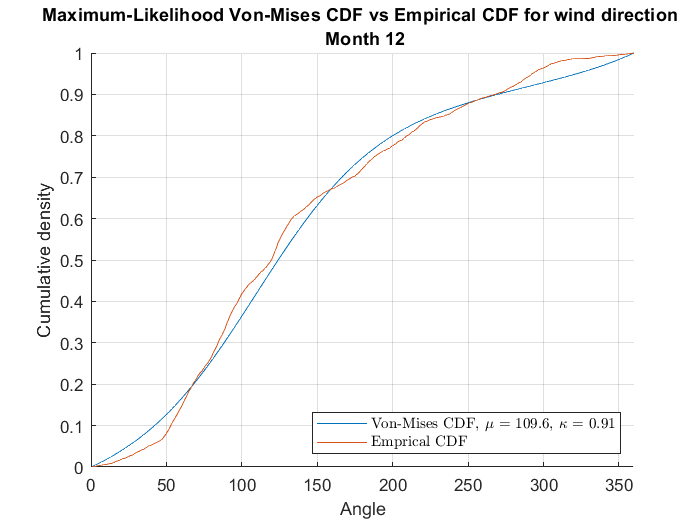
\includegraphics[ scale=0.5]{vm vs ecdf 41047 2019 december.png}
\caption{Mximum-Likelihood Von Mises CDF vs Empirical CDF, buoy 41047, Dec 2019}
\label{fig:41047 dec 2019}
\end{center}
\end{figure}

\begin{figure}[h!]
\begin{center}
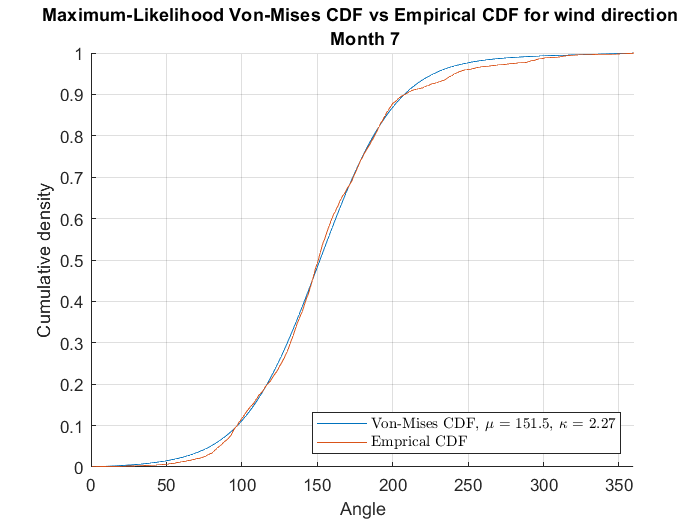
\includegraphics[ scale=0.5]{vm vs ecdf 41047 2019 july.png}
\caption{Mximum-Likelihood Von Mises CDF vs Empirical CDF, buoy 41047, July 2019}
\label{fig:41047 july 2019}
\end{center}
\end{figure}

Now that I can ingest data and fit distributions to it, my nest step will be to develop a model that can take these distributions and give reasonable simulated wind direction data. I will be relying on several different sources to aid me in my development, including \cite{Al Yammahi},\cite{Craig}, \cite{Kantilal}, and \cite{Rinaldo}, as well as others that I have not listed here. There is a significant body of work here and I have barely begun to scratch the surface of it. 



\begin{thebibliography}{1}

\bibitem{Al Yammahi} Aishah Al Yammahi \& Prashanth R. Marpu \& Taha B. M. J. Ouarda, ''Modeling directional distributions of wind data in the United
Arab Emirates at different elevations'', Arabian Journal of Geosciences, 2021

\bibitem{borradaile} Borradaile, G. J. (2003). Statistics of earth science data : their distribution in time, space, and orientation. Springer. ISBN 978-3-662-05223-5

\bibitem{Mahrt} Larry Mahrt, ''Surface Wind Direction Variability'',  Journal of Applied Meteorology and Climatology, 2011

\bibitem{Kantilal}Mardia, Kantilal; Jupp, Peter E. (1999). Directional Statistics. Wiley. ISBN 978-0-471-95333-3.

\bibitem{fisher} N.I. Fisher and A.J. Lee, ''Time Series Analysis of Circular Data'', Journal of the Royal Statistical Society. Series B, 1994

\bibitem{Craig} Peter S. Craig, ''Time Series Analysis for Directional Data'', Phd Thesis, 1988

\bibitem{Rinaldo} Rinaldo Artes \& Clelia M. C. Toloi (2009) An Autoregressive Model for Time
Series of Circular Data, Communications in Statistics - Theory and Methods, 39:1, 186-194, DOI:
10.1080/03610920802650338

\bibitem{Kaito} Shogo Kaito, ''A Markov process for circular data'', Journal of the Royal Statistical Society Series B, 2010
\end{thebibliography}



\end{document}